%****************************************************
%	CHAPTER 2 - Prototype Design
%****************************************************
\chapter{Prototype Design}
\label{ch:proto}
%====================================================
\section{Design}
\label{sec:proto.design}
%====================================================
\begin{figure}[htbp]
\centering
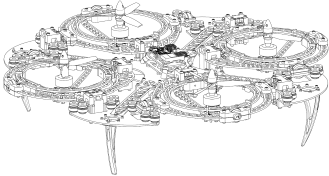
\includegraphics[width=0.93\textwidth]{figs/iso-design}
\caption{Isometric view of the prototype design}
\label{fig:iso-design}
\end{figure}
The final prototype (Fig:\ref{fig:iso-design}) went through a series of different design iterations, all aimed at optimizing engineering time spent on construction and reducing the associated component costs thereof. A significant aspect of consideration for the design process was the net weight whose upper limit, as mentioned before, is inherently limited by the thrust produced from lift motors. Some of the more important design factors, like inertias \& mass centers (Section:\ref{subsec:proto.design.inertia}), are discussed here in order to give context for the dynamics derived in the next chapter. The reference frame orientations which those dynamics are developed with respect to is then detailed as well. A brief overview of the electrical systems layout is given with the components associated and their electrical characteristics listed. Finally the actuator suite's functionality and transfer characteristics are also quantified. A review of the physical prototype realized and control loop implemented is detailed in Chapter:\ref{ch:flight}~along with actual flight test results.
\newpage
%====================================================
\subsection{Actuation}
\label{subsec:proto.design.actuation}
%====================================================
The novel component of the design is the manner of articulation for each concentric gimbal ring which forms the motor modules. The design objective is to produce a thrust vectoring actuation set for a quadrotor's control plant. The outcome was a module which independently redirects the thrust generated by the lift propellers (Fig:\ref{fig:motor-assembly}). Within each module are servos affixed onto sequential support rings to pitch and roll the substructure's axes. The gyroscope-like frame that surrounds each motor/propeller pair accommodates that relative movement. Aligned with each servo is a coaxial support bearing. The bearing and actuator servos have a mass disparity which results in an eccentric center of mass, producing a gravitational torque arm. Unfortunately, due to weight constraints, counter balance measures cannot be introduced. Consequences from the center of mass variations must be either compensated for (\emph{plant dependent solution}) or exploited in the dynamics (\emph{additional non-linear actuator plants}). The precise effects are quantified numerically next in Section:\ref{subsec:proto.design.inertia}.
\par
\begin{figure}[hbtp]
\begin{subfigure}{.5\textwidth}
\centering
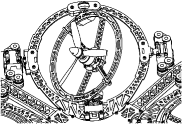
\includegraphics[width=\textwidth]{figs/motor-assembly}
\caption{Motor module assembly}
\label{fig:motor-assembly}
\end{subfigure}
\begin{subfigure}{.5\textwidth}
\centering
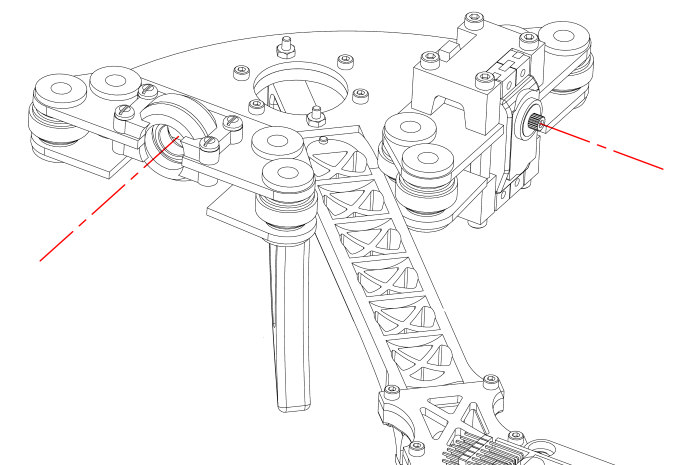
\includegraphics[width=\textwidth]{figs/motor-support}
\caption{Motor frame damping support assemblies}
\label{fig:motor_support}
\end{subfigure}
\caption{}
\end{figure}
Each motor module is positioned such that its produced thrust vector coincides with the intersection of its two rotational axes. As a result, there's only a perpendicular displacement co-planar to the body frames X-Y-Z origin (See Fig:\ref{fig:motor-frame}), $\vec{L}_{arm}$. That length directly affects the differential thrust torque $\tau_{diff}=\vec{L}_{arm}\times\vec{T}$. An off-center thrust vector line would make that arm displacement a non-orthogonal vector. The center of gravity for each module is time varying and depends on its two servo rotational positions. It's more practical to ensure intersection of the thrust vector with the rotational center than to balance the masses undergoing rotation. A thrust varying torque is harder to approximate and hence compensate for than a gravitational torque, given the complexity with modeling a propeller's aerodynamic thrust (Section:\ref{subsec:dynamics.aero.bem}).
\par
The primary body structure, similar to a traditional quadcopter '+' configuration, suspends each motor rotational assembly with silicon damping balls (Fig:\ref{fig:motor_support}). For damping to be effective there has to be roughly equatable relative masses between the two damped bodies. A smaller damping assembly in the center of the frame houses all the electronics and power distribution circuitry. All the mounting brackets which affix the motor module rings are 3D printed from CAD models using an Ultimaker V2+\cite{ultimaker}. There is a complete bill of materials for all parts used, including working drawings for each 3D printed bracket and the laser cut frame(s), in Appendix:\ref{app:bom}.
\par
\begin{figure}[hbtp]
\centering
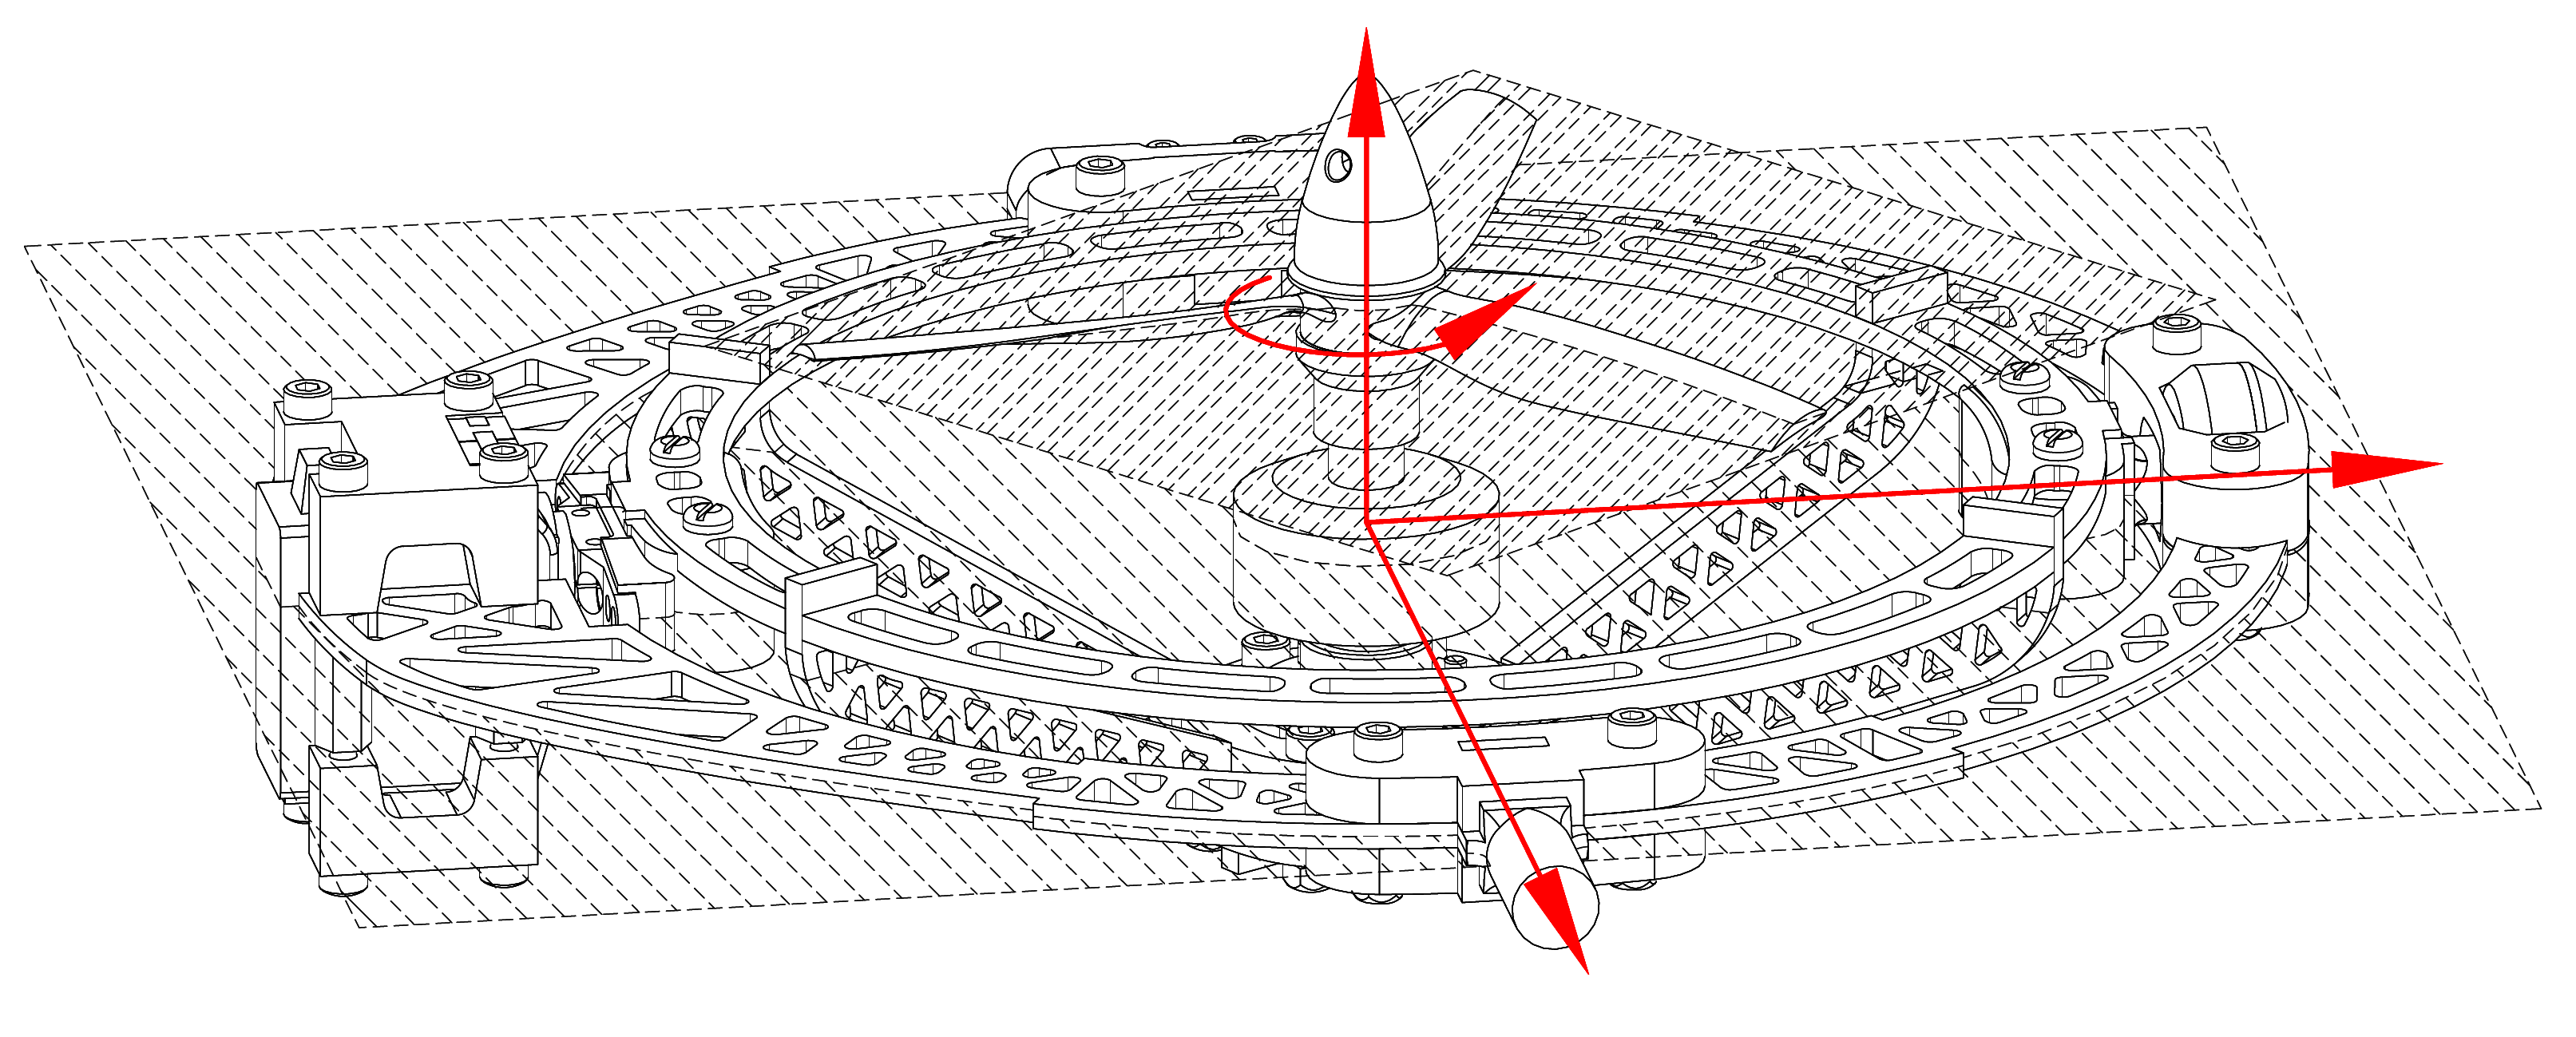
\includegraphics[width=0.9\textwidth]{figs/motor-prop}
\caption{Difference between propeller and motor planes}
\label{fig:motor_prop}
\end{figure}
The propellers rotational plane is not aligned exactly with the plane made by the $\hat{X}_{M_i}$ and $\hat{Y}_{M_i}$ rotational servo axes (Fig:\ref{fig:motor_prop}). The offset is approximately 23.39 mm and must be considered when evaluating pitch/roll gyroscopic torque responses later in Section:\ref{subsec:dynamics.nonlinearities.gyrotorques}. The propellers are 6 inch ($6 \times 4.5$) 3-Blade plastic Gemfam propellers, powered by Cobra CM2208-2000KV Brushless DC motors. The thrust produced as a function of angular velocity (in RPS) for the propellers is derived in Section:\ref{subsec:dynamics.aero.bem}. 
\newpage
The BLDC motors are controlled with LDPower 20A ESC\footnote{Flashed with BLHeli\cite{BLHeli} firmware} modules with an inline OrangeRx RPM Sensor. The transfer function for the combined unit is presented subsequently in Section:\ref{subsec:proto.design.transfer}. Power for the quadrotor is supplied not from a battery bank but from a power tether. Tethered power will ensure consistent flight time and reduce the concern of payload restriction on the available lift actuation. Power lines to both the BLDC motors and servos are supplied conventionally, however an ideal construction would see slip-rings for each module's power supply. 
\begin{figure}[htbp]
\centering
\begin{subfigure}{0.49\textwidth}
\centering
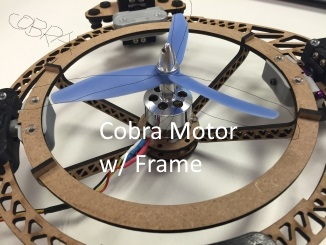
\includegraphics[width=0.9\textwidth]{figs/motor-bldc}
\caption{Cobra CM2208-2000KV BLDC Motor Module}
\label{fig:bldc-motor}
\end{subfigure}
\begin{subfigure}{0.49\textwidth}
\centering
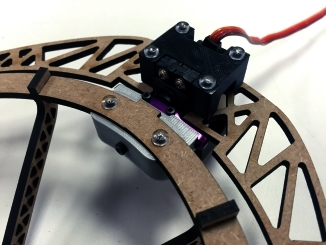
\includegraphics[width=0.9\textwidth]{figs/motor-servo}
\caption{Corona DS-339MG Servo Bracket}
\label{fig:motor-servo}
\end{subfigure}
\end{figure}
\par
Metal gear Corona DS-339MG digital servos are used for the two axes of rotation (Fig:\ref{fig:motor-servo}). Each servo has a range of 180\textdegree , positioned such that a $\text{zero}^{\text{th}}$ offset aligns the motor modules, adjacent to the body frame, and has a $\pm $90\textdegree range. A digital servo updates at 330 Hz, faster than a 50 Hz analogue servo equivalent (Table:\ref{tab:servo}). This means the otherwise $20$ms zero-order analogue sampling becomes a less significant $3.30$ms zero-order holding time. Both the $\hat{X}_{M_i}$ and $\hat{Y}_{M_i}$ axis servos will be rotating a large loading mass and so their \emph{open loop} plant dynamics are determined empirically in Section:\ref{subsec:proto.design.transfer} using test data included in Appendix:\ref{app:systemdat}.
\begin{table}[h]
\centering
\fbox{
\begin{minipage}{0.7\textwidth}
\begin{tikztimingtable}
50 Hz: &[C] 31{C} G\\
Analogue Servo &1{L} 1.5{H} 18.5{L} 1.5{H} 10{L}\\
Digital Servo&1{L} 15{1.5{H} 1.53{L}}\\
\end{tikztimingtable}
\end{minipage}
}
\caption{Analogue \& Digital Timing Signals}
\label{tab:servo}
\end{table}
%====================================================
\section{Conventions Used}
\label{sec:proto.conventions}
The attitude conventions used for the system's dynamic derivations, in the following Chapter:\ref{ch:dynamics},~are first briefly discussed here. Often these aspects are assumed to be obvious enough that they're omitted. It's important to clearly and unambiguously define a standard set of framing conventions to avoid uncertainty later. Rotation matrices are included but the focus is on the \emph{contrast} between a rotation and transformation operation. Both \cite{spacecraftattitutdequaternions} and \cite{rigidbodylecture} provide an in depth and thorough explanation of rotation matrices and DCM attitude representation if such concepts are unfamiliar to the reader. Quaternions are introduced in Section:\ref{subsec:dynamics.rigidbody.quaternion}.
%====================================================
\subsection{Reference Frames Convention}
\label{subsec:proto.conventions.frames}
%====================================================
\begin{figure}[htbp]
\centering
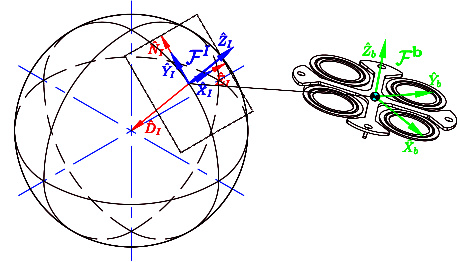
\includegraphics[width=0.65\textwidth]{figs/reference-frame}
\caption{Inertial and Body Reference Frames}
\label{fig:ref_frame}
\end{figure}
Euler (aerospace) frames are used for principle inertial and body coordinate representation (Fig:\ref{fig:ref_frame}). The inertial frame,~$\mathcal{F}^I$, is aligned such that the $\hat{X}_I$ axis is in the $\hat{N}$orth direction, $\hat{Y}_I$ is in the $\hat{E}$ast direction and $\hat{Z}_I$ is  in the $\hat{D}$ownward direction\footnote{In orbital sequences this would be toward the Earth's center. Sometimes referred to as the N\^{E}D convention}. The body frame, $\mathcal{F}^b$, then has both $\hat{X}_b$ and $\hat{Y}_b$ aligned obliquely between two perpendicular arms of the quadrotor's body and the $\hat{Z}_b$ axis in the body's normal direction (Fig:\ref{fig:body-frame}). The body frame's axes and their relation to the prototype design are highlighted next in Section:\ref{subsec:proto.conventions.motoraxis}. Frame superscripts $I$ and $b$ represent inertial and body frames respectively whilst vector subscripts imply the reference frame in which the vector's coordinates exists or taken relative to.
\par
Relative angular displacement between two frames is commonly measured by the three angle Euler set. The Euler angles $\vec{\eta}=[\phi ~\theta ~\psi]^T$ represents rotations about the $\hat{X}$,$\hat{Y}$ and $\hat{Z}$ axes respectively. Depending on how the rotation sequence is formulated, those angles can be used to construct rotation matrices which give relation to vectors or can transform coordinates. The generic equation to \emph{rotate} a vector $\vec{v}$ about a (normalized) axis $\hat{n}$ by some angle $\mu$ is given by\footnote{Derived and proven in \emph{Quadrotor Dynamics and Control}\cite{quaddynamics}}:
\begin{equation}\label{eq:genrotationmatrix}
\vec{v}~'=\big(1-cos(\mu)\big)\big(\vec{v}\cdot \hat{n}\big)\hat{n}+cos(\mu)\vec{v}+sin(\mu)\big(\hat{n}\times\vec{v}\big)
\end{equation}
Which, when $\hat{n}$ is either $\hat{X}$,$\hat{Y}$ or $\hat{Z}$ axes, can be simplified to produce the fundamental rotation matrices $\mathbb{R}_x(\phi)$,$\mathbb{R}_y(\theta)$ and $\mathbb{R}_z(\psi)$.
\newpage
Multiplication by a rotation matrix $\mathbb{R}(\cdot)$ applies a left-handed \emph{rotation} operator, the resultant vector still exists in the same reference frame. An $\hat{X}$ axis rotation by $\phi$ is;
\begin{subequations} \label{eq:rotationoperator}
\begin{equation}\label{eq:rotationoperator.a}
\vec{v}~'=\mathbb{R}_{x}(\phi)\vec{v}
\end{equation}
\vspace{-15pt}
\begin{equation}\label{eq:rotationoperator.b}
\vec{v}~',\vec{v}\in\mathcal{F}^1
\end{equation}
\end{subequations}
\emph{\color{Gray} No subscripts are used in Eq: \ref{eq:rotationoperator} to indicate reference frame ownership because all vectors are in the same frame}
\par
A vector \emph{transformation} changes the resultant vector's reference frame. Transformation is then a rotation by an angle of the \emph{difference} between the resulting and principle reference frames. A transformation from frame $\mathcal{F}^1$ to $\mathcal{F}^2$, differing by an angle of $\phi$ about the $\hat{X}$ axis is then:
\begin{subequations}\label{eq:transformationoperator}
\begin{equation}\label{eq:transformationoperator.a}
\vec{v}_2=\mathbb{R}_x(-\phi)\vec{v}_1
\end{equation}
\vspace{-15pt}
\begin{equation}\label{eq:transformationoperator.b}
\vec{v}_2\in\mathcal{F}^2~\text{and}~\vec{v}_1\in\mathcal{F}^1
\end{equation}
\end{subequations}
The distinction between Eq:\ref{eq:rotationoperator} and Eq:\ref{eq:transformationoperator} is the directional sense of the angular operand $\phi$, and hence the effect it has on the argument vector. The transformation or rotation of a vector from $\mathcal{F}^I$ to $\mathcal{F}^b$ is the product of three sequential operations about each axis. Each subsequent rotation is applied relative to a new intermediate frame; hence each Euler angle is taken relative to a specific intermediate frame. The sequence of axial rotation operations does indeed effect the Euler set. Any consequences of that chosen order is something discussed indepth in \emph{Quaternions and Rotation Sequence}, \cite{rotationsequences}. In this dissertation the Z-Y-X sequence is used. A transformation of the vector $\vec{v}$ from the inertial to the body frame is then applied by:
\\
\begin{subequations}
\begin{equation}\label{eq:inertialbodytransformation.a}
\mathbb{R}_{I}^{b}\triangleq\mathbb{R}_z(\psi)\mathbb{R}_y(\theta)\mathbb{R}_x(\phi)
\end{equation}
\vspace{-10pt}
\begin{equation}\label{eq:inertialbodytransformation.b}
\vec{v}_b=\mathbb{R}_I^b(-\psi,-\theta,-\phi)\vec{v}_I
\end{equation}
\vspace{-10pt}
\begin{equation}\label{eq:inertialbodytransformation.c}
\Rightarrow\vec{v}_b=\mathbb{R}_z(-\psi)\mathbb{R}_y(-\theta)\mathbb{R}_x(-\phi)\vec{v}_I
\end{equation}
\vspace{-10pt}
\begin{equation} \label{eq:inertialbodytransformation.d}
\mathbb{R}_z(-\psi)\mathbb{R}_y(-\theta)\mathbb{R}_x(-\phi) \iff \mathbb{R}_x(\phi)\mathbb{R}_y(\theta)\mathbb{R}_z(\psi)=\mathbb{R}_{b}^{I}
\end{equation}
\vspace{-10pt}
\begin{equation}
\mathbb{R}_I^b=\big(\mathbb{R}_b^I\big)^{-1}=\big(\mathbb{R}_b^I\big)^T
\end{equation}
\end{subequations}
The relationship in Eq:\ref{eq:inertialbodytransformation.d} is an inversion (\emph{transpose}) of the rotation matrix. A rotation matrix's inverse can be used interchangeably with its negative counterpart to maintain a positive sense of the argument angle. To ensure clarity throughout this dissertation's mathematics, a negative angular sense implies a \emph{transformation} to a different reference frame. Where applicable, the order of rotation will indicate the sequence direction and an angular sign differentiates the rotation and transformation operators.
\par
The body frame's angular velocity is taken relative to the inertial frame, represented by $\vec{\omega}_{b/I}\Rightarrow \vec{\omega}_b$. Seeing that each Euler angle is measured with respect to an intermediary frame, a distinction must then be made between $\dot{\eta}$ and $\vec{\omega}_b$. All three Euler angles need to be transformed to one common frame. Exploiting vehicle frames 1 \& 2, or rather $\mathcal{F}^{v1}$ \& $\mathcal{F}^{v2}$, as intermediate frames to respectively describe post $\mathbb{R}_x(\phi)$ and $\mathbb{R}_y(\theta)$ operations.
\begin{subequations}
\begin{equation}\label{eq:angular-rates.a}
\vec{\omega}_b=\frac{d}{dt_b}\eta=\frac{d\phi}{dt}\mathbb{R}_{v2}^b(\phi)\begin{bmatrix}
\phi\\
0\\
0\\
\end{bmatrix}
+
\frac{d\theta}{dt}\mathbb{R}_{v2}^{b}(\phi)\mathbb{R}_{v1}^{v2}(\theta)\begin{bmatrix}
0\\
\theta\\
0
\end{bmatrix}
+
\frac{d\psi}{dt}\mathbb{R}_{v2}^{b}(\phi)\mathbb{R}_{v1}^{v2}(\theta)\mathbb{R}_{I}^{v1}(\psi)\begin{bmatrix}
0\\
0\\
\psi
\end{bmatrix}
\end{equation}
\emph{\color{Gray}The vehicle frames in Eq:\ref{eq:angular-rates.a} and the subsequent rotations between each frame don't necessarily have to be in that order. The equation could change depending on what rotation sequence was used.}
\newpage
Which then simplifies to the formal relationship between two rotating frames, with $\vec{\omega}_b=[p~q~r]^T$ in $rad.s^{-1}$:
\begin{equation}\label{eq:angular-rates.b}
\begin{bmatrix}
p\\
q\\
r\\
\end{bmatrix}
=
\begin{bmatrix}
1 & 0 & -sin(\theta)\\
0 & cos(\phi) & sin(\phi)cos(\theta)\\
0 & -sin(\theta) & cos(\phi)sin(\theta)\\
\end{bmatrix}
\begin{bmatrix}
\dot{\phi}\\
\dot{\theta}\\
\dot{\psi}\\
\end{bmatrix}
\end{equation}
\vspace{-10pt}
\begin{equation}\label{eq:angular-rates.c}
\Rightarrow\vec{\omega}_b=\Psi(\eta)\dot{\eta}
\end{equation}
\vspace{-10pt}
\begin{equation}\label{eq:angular-rates.d}
\Psi(\eta)=
\begin{bmatrix}
1 & 0 & -sin(\theta)\\
0 & cos(\phi) & sin(\phi)cos(\theta)\\
0 & -sin(\theta) & cos(\phi)sin(\theta)\\
\end{bmatrix}
\end{equation}
\vspace{-5pt}
\begin{equation}\label{eq:angular-rates.e}
\Rightarrow\dot{\eta}=\Psi^{-1}(\eta)\vec{\omega}_b=\Phi(\eta)\vec{\omega}_b
\end{equation}
\vspace{-10pt}
\begin{equation}\label{eq:angular-rates.f}
\Phi(\mathcal{E})=\begin{bmatrix}
1 & sin(\phi)tan(\theta) & cos(\phi)tan(\theta)\\
0 & cos(\phi) & -sin(\phi)\\
0 & sin(\phi)sec(\theta) & cos(\phi)sec(\theta)\\
\end{bmatrix}
\end{equation}
\end{subequations}
\par
The termed \emph{Euler} matrix, $\Phi(\eta)$, contains a well known and problematic singularity at $\theta=\pm\pi/2$; because $sec(\theta)\rightarrow\infty$ as $\theta\rightarrow\pi/2$. The effect of the rotation matrix singularity is further explored later in Section:\ref{subsec:dynamics.rigidbody.singularity}. It's manifestation in the $\theta$ angle here is a direct consequence of the Z-Y-X sequence used. Each Euler angle can potentially suffer a singularity depending on how the rotations are sequenced. Indeed quaternions are used for kinematics later in lieu of Euler angles. Euler angular attitude representation is, however, easily understood and well suited to the conventional distinctions made in this Chapter.
\par
Quaternion operations are similarly sequenced in the Z-Y-X order:
\begin{subequations}
\begin{equation}\label{eq:quaternion-rotation-equivalence}
\mathbb{R}_I^b\iff Q_b \otimes (.) \otimes Q_b^*
\end{equation}
\vspace{-15pt}
\begin{equation}
Q_b \triangleq Q_z Q_y Q_x~\text{and}~Q_b \triangleq Q_x^* Q_y^* Q_z^*
\end{equation}
\end{subequations}
With $\otimes$ being the Hamilton product (or quaternion multiplication). Each quaternion, $Q_i$, is a unit quaternion about that $\hat{i}^{th}$ axis. It is important to note that a quaternion rotation operates on an argument vector with a zero quaternion scalar component. So then for some vector $\vec{v}$, the quaternion rotation operation in Eq:\ref{eq:quaternion-rotation-equivalence} is equivalent to;
\begin{subequations}
\begin{equation}\label{eq:quaternion-operator.a}
Q_{\vec{v}}~'=Q \otimes (Q_{\vec{v}}) \otimes Q^*
\end{equation}
\vspace{-10pt}
\begin{equation}\label{eq:quaternion-operator.b}
\text{Where}~Q_{\vec{v}}=\begin{bmatrix}
0\\
\vec{v}\\
\end{bmatrix},~Q_{\vec{v}~'}=\begin{bmatrix}
0\\
\vec{v}~'\\
\end{bmatrix}
\end{equation}
\end{subequations}
The quaternion representation in Eq:\ref{eq:quaternion-operator.b} ensures that the operation is entirely in $\mathbb{R}^4$ space. However it is usually omitted, despite $\mathbb{R}^4$ being implied and as such, Eq:\ref{eq:quaternion-operator.a} is then simply:
\begin{equation}
\vec{v}~'=Q \otimes (\vec{v}) \otimes Q^*
\end{equation}
Quaternion dynamics, and the quaternion operator, are later expanded upon to replace the use of Euler angles and Rotation matrices as a convention for attitude representation later in Chapter:\ref{ch:dynamics}
\newpage
%====================================================
\subsection{Motor Axis Layout}
\label{subsec:proto.conventions.motoraxis}
%====================================================
Fundamentally the whole structure, although treated as fixed and rigid in the kinematics, consists of multiple rigid bodies with relative rotations to one another, illustrated previously in the design description in Section:\ref{sec:proto.design}. Those rigid bodies are divided into four inter-connected motor modules and a single body structure. Each module consists of two sequential gimbal rings, each with one degree of relative rotation between itself and the next subsequent ring. There needs to be distinct nomenclature used for describing these motor modules. 
\begin{figure}[htbp]
\centering
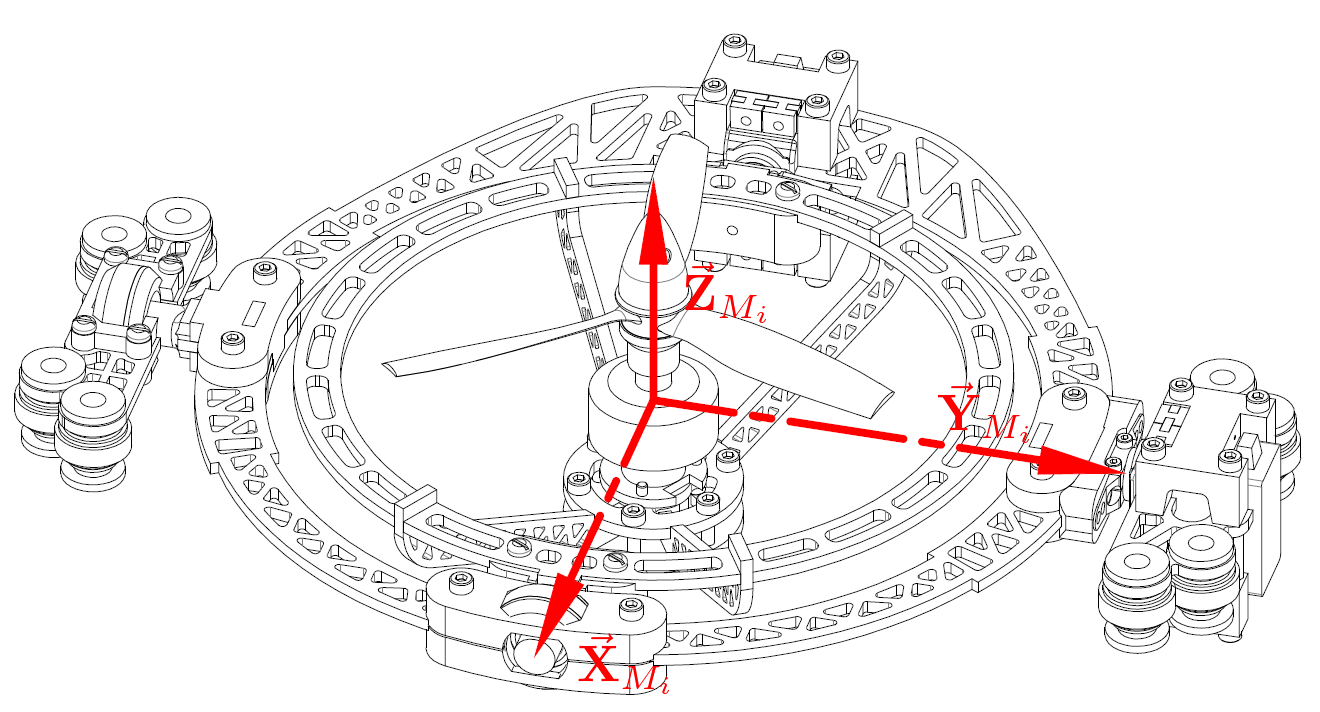
\includegraphics[width=0.85\textwidth]{figs/motor-axes}
\caption{Aligned Motor Frame Axes}
\label{fig:motor-axes}
\end{figure}
\par
Every propeller/motor pair is actuated by two servos. The $i^{th}$ propeller, directly driven by the motor's rotor, has a rotational speed $\Omega_i~[RPS]$ about the $\hat{Z}$ stator axis. Two servos are aligned \emph{at rest} with $\hat{Y}$ and $\hat{X}$ axes to pitch and roll the propeller away from its principle rotational axis. Each motor has its own reference frame, $\mathcal{F}^{M_i}$, aligned in Fig:\ref{fig:motor-axes} and highlighted with the rotational rings in Fig:\ref{fig:motor-frame}.
\par
\begin{minipage}{\textwidth}
\begin{wrapfigure}{r}{0.55\textwidth}
\centering
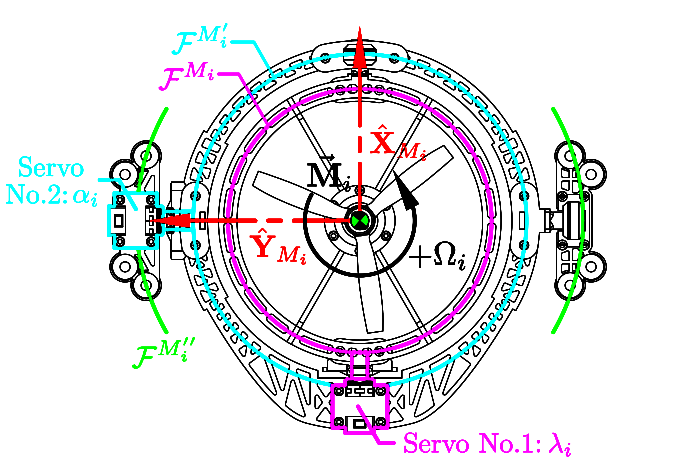
\includegraphics[width=0.55\textwidth]{figs/motor-frame}
\caption{Intermediate Motor Frames}
\label{fig:motor-frame}
\end{wrapfigure}
Motor frames, numbered $1-4$, transform to the body frame first by an angle of $\lambda_i$\textdegree ~about the $\hat{X}_{M_i}$ axis. Then by $\alpha_i$\textdegree ~about the $\hat{Y}_{M_i'}$ axis in an intermediate $M_i'$ frame. The first servo actuates $\lambda_i$, rotating $\mathcal{F}^{M_i}$ to an intermediate $\mathcal{F}^{M_i'}$ frame. Secondly, the next servo actuates $\alpha_i$ to produce a second intermediate frame $M_i''$. That second servo is affixed in the $M_i''$ frame. Lastly there's a relative orthogonal rotation about $\hat{Z}_{M_i''}$ between $\mathcal{F}^b$ and $\mathcal{F}^{M_i''}$. Each module's actuation state is fully described by $[\Omega_{i},~\lambda_{i},~\alpha_{i}]^{T}$ for $i\in [1:4]$. The four motor modules are aligned relative to the body's XYZ axes as shown in Fig:\ref{fig:body-frame}. Modules 1 and 3 have their X-axes in the positive and negative $\hat{X}$ directions of the body frame respectively. Similarly Modules 2 and 4 have their X-axes in the positive and negative $\hat{Y}$ directions of the body frame.
\end{minipage}
\newpage
\begin{figure}[htbp]
\centering
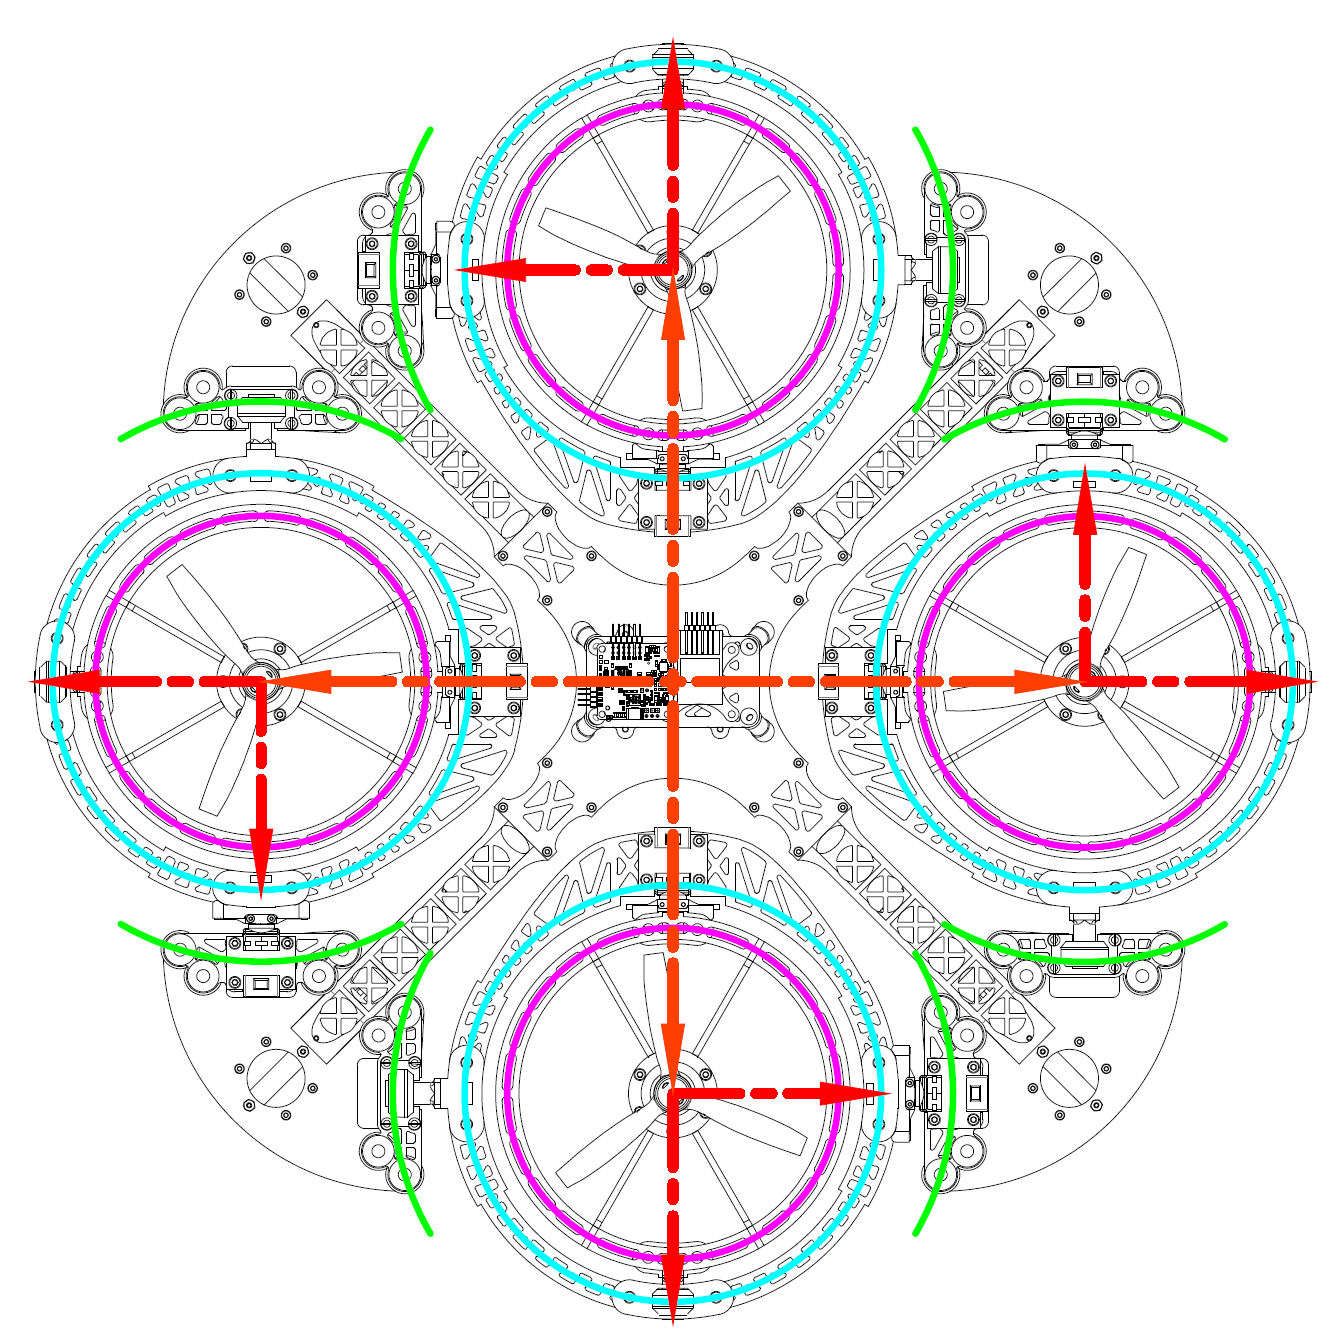
\includegraphics[width=0.9\textwidth]{figs/body-frame}
\caption{Body Frame Axes Layout}
\label{fig:body-frame}
\end{figure}
\par
\emph{\color{Gray}Not shown in Fig:\ref{fig:body-frame} is the relative $\hat{Z}$ axis position with respect to the structure. The $\hat{Z}$ height of the body's motion centroid is such that its origin is co-planar with the four motor modules rotational centers. The center of motion is \underline{not} the center of mass, an aspect which is investigated next in Section:\ref{subsec:proto.design.inertia}.}
\\
Vector transformations from each of the motor frames to the body frame are characterized as:
\begin{subequations}
\begin{equation}\label{eq:motor-module-rotation.a}
\vec{v}_b=\mathbb{R}_z(-\sigma_i)\mathbb{R}_y(-\alpha_i)\mathbb{R}_x(-\lambda_i)\vec{v}_{M_i},~\sigma_i\in[0, 90^{\circ}, 180^{\circ}, 270^{\circ}]
\end{equation}
With orthogonal rotation matrices $\mathbb{R}_z$:
\begin{equation}\label{eq:motor-module-rotation.b}
\mathbb{R}_z=\begin{bmatrix}
1 & 0 & 0\\
0 & 1 & 0\\
0 & 0 & 1
\end{bmatrix}, \begin{bmatrix}
0 & -1 & 0\\
1 & 0 & 0\\
0 & 0 & 1
\end{bmatrix}, \begin{bmatrix}
-1 & 0 & 0\\
0 & -1 & 0\\
0 & 0 & 1
\end{bmatrix}, \begin{bmatrix}
0 & 1 & 0\\
-1 & 0 & 0\\
0 & 0 & 1
\end{bmatrix}~\text{for}~i\in[1,2,3,4]~\text{respectively}
\end{equation}
\label{eq:motor-module-rotation}
\end{subequations}
\\
The entire actuator space, including propeller speed $\Omega_i~[RPS]$, is then $\in\mathbb{R}^{12}$, or rather $\mathbb{U}\in\mathbb{R}^{12}$. The actuator input set $u \in \mathbb{U}$ is then structured as:
\begin{equation}
u_{\in\mathbb{U}}=\big[ \Omega_{1} ~ \lambda_{1} ~ \alpha_{1} ~ \ldots ~ \Omega_{4} ~ \lambda_{4} ~ \alpha_{4}  \big]^T
\end{equation}
\newpage
%====================================================
\subsection{Inertial Matrices \& Mass}
\label{subsec:proto.design.inertia}
%====================================================
\emph{\color{Gray} Although inertias are presented here rounded to either 2 or 0 decimal places, full floating point numbers are used in simulation and prototype software. Un-rounded inertias are included in Appendix:\ref{app:eq}. Similarly rotation matrices produce a more cumbersome results for Eq:\ref{eq:inertia.middle},\ref{eq:module-inertia},\ref{eq:body-net}, which are all  susceptible to singularities. Quaternion transformations between rotating reference frames are used in practice.}
\subsubsection*{Inertias}
An undesirable side effect of the relative rigid body rotations within the structure are the inertial responses produced associated with such movements. Given Newton's Second Law of Rotational Motion$^{\dagger}$, each applied rotation is going to produce an equal but opposite reaction onto the principle inducing frame. Similarly a gyroscopic cross product from rotational velocities is also present. Such first and second order effects are often neglected given that the angular rates which they're dependent on are mostly small enough to approximate as zero, $\vec{\omega}_b\approx\vec{0}$. A dynamic set-point (non-zero) attitude tracking plant is, however, going to produce sizeable time varying body angular velocities and accelerations. Unlike a traditionally actuated quadrotor, such effects have to be accounted for.
\begin{figure}[htbp]
\centering
\begin{subfigure}{0.49\textwidth}
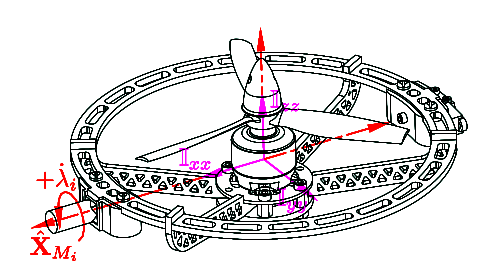
\includegraphics[width=\textwidth]{figs/inertia-inner}
\caption{Inner Ring Rotational Structure}
\label{fig:inertia-inner}
\end{subfigure}
\begin{subfigure}{0.49\textwidth}
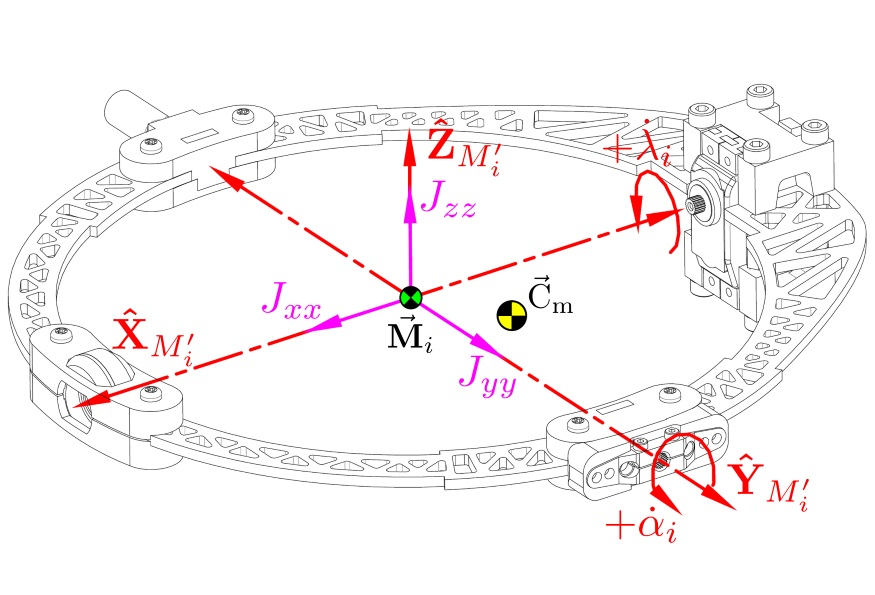
\includegraphics[width=\textwidth]{figs/inertia-middle}
\caption{Middle Ring Rotational Structure}
\label{fig:inertia-middle}
\end{subfigure}
\caption{Inertial Measurement References}
\end{figure}
\par
The manifestation of the aforementioned torques are explored in thorough detail in Section:\ref{sec:dynamics.nonlinearities}. Those effects are both dependent on the rotational body's inertial tensor\footnote{All inertias are assumed symmetrical and calculated in Solidworks with overridden masses to match physical prototype measurements, all those values are included in Appendix:\ref{app:bom}} about each respective rotational axis. The magnitude of those inertias are obviously a by-product of the structure's design. Starting with the innermost assembly, in each Motor Frame $\mathcal{F}^{M_i}$, the inner ring structure is a 92g assembly (all components incorporated). The rotational center \emph{roughly} coincides with the center of its mass ($C.M=[-1.44~0 ~5.81]^T~~[mm]$ relative to its rotational center). The inner ring being rotated by $\lambda_i$\textdegree ~about the $\hat{X}_{M_i}$ axis then has an inertial matrix (centered and aligned with axes as in Fig:\ref{fig:inertia-inner}):
\begin{subequations}\label{eq:inertia.inner}
\begin{equation} \label{eq:inertia.inner.a}
\mathbb{I}_{M_i}=\begin{bmatrix}
561.96 & -32.29	& -0.26\\
-32.29 & 1888.74 & 0.00\\
-0.26 & 0.00	& 2090.97\\
\end{bmatrix}~~[g.cm^2]
\end{equation}
\vspace{-5pt}
\begin{equation} \label{eq:inertia.inner.b}
\approx diag\big(562, ~1889, ~2091\big)\times10^{-7}~~[kg.m^2]
\end{equation}
\end{subequations}
The effect of rapidly spinning propellers on the inertia in Eq:\ref{eq:inertia.inner.a} is approximated well by a solid disc, hence the inner ring's inertial components are regarded as constant. The moment of inertia about that $\hat{X}_{M_i}$ rotational axis, pertinent to a $\lambda_i$ rotation, is then $\mathbb{I}_{\lambda}\approx 531\times10^{-7}~~[kg.m^2]$.
\par
The first $\lambda_i$ actuating servo and bearing supports are affixed to the intermediate middle ring assembly (Fig:\ref{fig:inertia-middle}). The middle ring frame, $\mathcal{F}^{M_i'}$, is a $98g$ structure, excluding the inner most ring. Collectively the mass for both the inner and middle rings structures is $m_{module}=190g$. The middle ring is rotated by $\alpha_i$\textdegree ~about its $\hat{Y}_{M_i'}$ axis. The compound body's inertia about that axis of rotation, $\hat{Y}_{M_i}$, is a combination of both the middle ring's inertia and the inner ring's.  The latter contribution being a function of the \emph{rotation} (not transformation) angle $\lambda_i$\textdegree ~which, from the conservation of angular momentum theory \cite{rigidbodyinertia}\footnote{$\mathbb{R}_x$ is a full rank and square, so an inverse $\mathbb{R}^{-1}_{x}$ always exists}, is:
\begin{subequations}\label{eq:inertia.middle}
\begin{equation} \label{eq:inertia.middle.a}
\text{If} ~~\mathbb{I}_{middle}=\begin{bmatrix}
2905.70 & 0.02 & 390.89\\
0.02 & 8446.41 & 0.01\\
390.89 & 0.01 & 11125.74\\
\end{bmatrix}~~[g.cm^2]
\end{equation}
\vspace{-5pt}
\begin{equation}\label{eq:inertia.middle.b}
\mathbb{I}_{M_i'}=\mathbb{I}_{middle}+\mathbb{R}_{x}(\lambda_i)\big(\mathbb{I}_{inner}\big)\mathbb{R}_{x}^{-1}(\lambda_i)
\end{equation}
\vspace{-10pt}
\begin{equation}\label{eq:inertia.middle.c}
\mathbb{I}_{M_i'}(\lambda_i)=\mathbb{I}_{const}+\mathbb{I}_{M_i}(\lambda_i)
\end{equation}
\vspace{-10pt}
\begin{equation} \label{eq:inertia.middle.d}
\approx\begin{bmatrix}
3468 & 0 & 391\\
0 & 10436 & 0\\
391 & 0 & 13155\\
\end{bmatrix}
+
\begin{bmatrix}
0 & -32{c}_{\lambda} & -32{s}_{\lambda}\\
-32{c}_{\lambda} & -101{c}_{2\lambda} & 101s_{2\lambda}\\
-32{s}_{\lambda} & 101s_{2\lambda} & 101{c}_{2\lambda}\\
\end{bmatrix}
\times10^{-7}~~[kg.m^2]
\end{equation}
\end{subequations}
With $\mathbb{I}_{inner}=\mathbb{I}_{M_i}$ being the inertia from Eq:\ref{eq:inertia.inner.a}, re-orientated with a rotation $\mathbb{R}_x(\lambda_i)$. The net inertia is then a function of the rotation angle $\lambda_i$ and a constant inertia (Eq:\ref{eq:inertia.middle.c}) which is then simplified\footnote{Eq:\ref{eq:inertia.middle.d} is rounded to no decimal places, seeing that its units are already $\times10^{-7}$ and thus some products of inertia are omitted.} to Eq:\ref{eq:inertia.middle.d}. It's important to note the two non-zero products of inertia, $\mathbb{I}_{yx}$ and $\mathbb{I}_{yz}$, which are going to result in a vector $\vec{\tau}_\eta$ response. The inertia then encountered by an $\alpha_i$ rotation is:
\begin{equation}\label{eq:inertia.middle.vpa}
\mathbb{I}_\eta(\lambda)\approx[-32{c}_{\lambda},~ 10436-101{c}_{2\lambda},~ 101{s}_{2\lambda}]^T\times10^{-7}~~[kg.m^2]
\end{equation}
\par
Variable inertias dependent on state input variables are the first of many non-trivial aspects unique to this aircraft's design. The resultant control solutions are thus decidedly plant dependent in their formulation. Secondly, the center of mass for the motor module's compound assembly isn't coincidental with either rotational axes intersection. As a result the effective center of mass for the entire structure is going to be a function of the angular rotational position of each motor module and time varying.
\par
\begin{figure}[htbp]
\centering
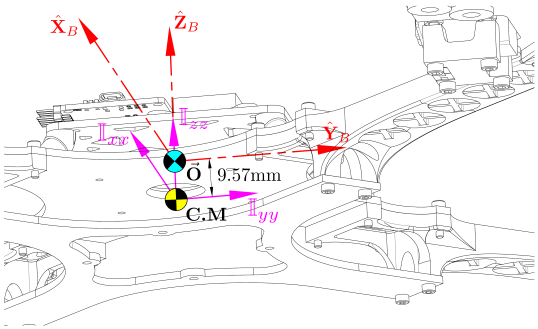
\includegraphics[width=0.8\textwidth]{figs/inertia-center}
\caption{Body Frame Center of Mass}
\label{fig:inertia-center}
\end{figure}
The second $\alpha_i$ rotating servo adjoins the complete motor module (both the inner and middle ring assemblies) to the body structure. The inertial volume of the servo and bearing supports contribute then to the body structure's inertia, whose value excludes any of the four motor modules. Consisting of servo and bearing damping brackets, each "damping" assembly collectively weighs $84g$ and suspends the motor modules from the body frame with a set of silicon damping balls. The body structure's center of mass (without motor modules, Fig:\ref{fig:inertia-center}) coincides with the XY directional axes and lies $\Delta Z=-9.57~mm$ below the Body Frame's origin of motion, $\vec{O}\in\mathcal{F}^b$.
\\
\emph{\color{Gray}Note: the origin which all motion is calculated with respect to is co-planar to the motor module's rotational centers, \underline{not} the net center of mass.}
\\
The body's weight, including all four damping assemblies and electronics, totals to $814.7~g$. The body's net inertia (\emph{sans} motor modules) $\mathbb{I}_{body}$, about its center of mass is (Fig:\ref{fig:inertia-center})
\begin{subequations}\label{eq:inertia.body}
\begin{equation}\label{eq:inertia.body.a}
\mathbb{I}_{body}=\begin{bmatrix}
181689.67 & -0.44 & -8.86\\
-0.44 & 181567.22 &	-19.44\\
-8.86 & -19.44 & 360077.58\\
\end{bmatrix}\times 10^{-7}~~[kg.m^2]
\end{equation}
Using the Parallel Axis theorem$^{\dagger}$, that same net body inertia about the body frame's origin, $\vec{O}_b$, is:
\begin{equation}\label{eq:inertia.body.b}
{\mathbb{I}_{body}}'=\mathbb{I}_{body}+m(\vec{d}\cdot\vec{d}+\vec{d}\otimes\vec{d})\approx\mathbb{I}_{body}+md^2
\end{equation}
\emph{\color{Gray}Here $\otimes$ represents the Hamilton product of two 3X3 matrices, it's used again later in Chapter:\ref{ch:dynamics} to indicate the quaternion multiplication operator.}
\begin{equation}\label{eq:inertia.body.b}
\underset{\vec{\mathbf{O}}}{{\mathbb{I}_{body}}'}=\begin{bmatrix}
182435.66 & -0.42 & -6.46\\
-0.42 & 182313.18 & -14.52\\
-6.46 & -10.41 & 360077.62\\
\end{bmatrix} \times10^{-7}~[kg.m^2]
\end{equation}
\end{subequations}
Net inertia for the compound assembly, $\mathbb{I}_b$\footnote{Disambiguation: $\mathbb{I}_b$ is \emph{net} body frame's inertia, different from $\mathbb{I}_{body}$ which is the inertia for \emph{just} the body structure}, about the origin $\vec{O}_b$ is a combination of all the relative attached bodies. That being; the four motor modules, transformed and then translated to the center of motion, and the body structure itself. That transformation is analogous to that of Eq: \ref{eq:motor-module-rotation}. Reiterating that the the origin is co-planar to the module's center of rotation, each motor module's inertia, $\mathbb{I}_{M_i'}$\footnote{As defined in Eq:\ref{eq:inertia.middle.d}}, is further rotated by $\alpha_{i}$\textdegree ~about $\hat{Y}_{M_i'
}$ and finally an orthogonal $\hat{Z}_{M_i''}$ rotation (aligned with $\hat{Z}_b$) onto $\mathcal{F}^b$. Still measured with respect to their individual rotational centers, $\vec{\mathbf{M}}_i$, but re-orientated to align with $||\vec{\mathbf{O}}_b$. Contribution of each motor module's inertia, with $\mathbb{R}_z$ being the same as Eq:\ref{eq:motor-module-rotation.b}, is then:
\begin{subequations}\label{eq:module-inertia}
\begin{equation}\label{eq:module-inertia.a}
\mathbb{I}_{i^{th} motor}=\mathbb{R}_{z}(\sigma_i)\mathbb{R}_{z}(\alpha_i)\big(\mathbb{I}_{M_i'}(\lambda_i)\big)\mathbb{R}^{-1}_{y}(\alpha_i)\mathbb{R}^{-1}_{z}(\sigma_i)
\end{equation}
Expanding to Inner and Middle Ring components:
\begin{equation}\label{eq:module-inertia.b}
=\mathbb{R}_{z}\mathbb{R}_{y}(\alpha_i)\big(\mathbb{I}_{middle}\big)\mathbb{R}^{-1}_{y}(\alpha_i)\mathbb{R}^{-1}_z+\mathbb{R}_{z}\mathbb{R}_{y}(\alpha_i)\mathbb{R}_{x}(\lambda_i)\big(\mathbb{I}_{inner}\big)\mathbb{R}^{-1}_{x}(\lambda_i)\mathbb{R}^{-1}_{y}(\alpha_i)\mathbb{R}^{-1}_z
\end{equation}
\vspace{-10pt}
\begin{equation}\label{eq:module-inertia.b}
\text{With axes}~\hat{X}\in\mathcal{F}^{M_i},~~\hat{Y}\in\mathcal{F}^{M_i'},~~\hat{Z}\in\mathcal{F}^{M_i''}
\end{equation}
\end{subequations}
\emph{\color{Gray}It's at this stage that, despite simplifications, the symbolic inertial equation becomes overly cumbersome to include with numeric values\ldots For the sake of brevity, exact calculated inertial values for the input dependent plant are omitted.}
\par
\begin{figure}[hbtp]
\centering
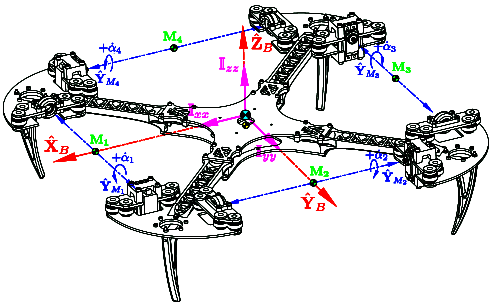
\includegraphics[width=0.9\textwidth]{figs/inertia-frame}
\caption{Inertial Center \& Mass Center}
\label{fig:inertia-frame}
\end{figure}
Each module's rotational center ($[\pm 195.16~0~0]$ \& $[0~\pm 195.16~0]$ recalling Fig:\ref{fig:body-frame}) are spaced equally relative to $\vec{\mathbf{O}}_b$ with a parallel axis arm $\vec{L}_{arm}=\begin{bmatrix}
195.16 & 0 & 0
\end{bmatrix}^T~~[mm]$ (Fig:\ref{fig:inertia-frame}). The net inertial equation about $\vec{\mathbf{O}}_b$, dependent on the actuator suite $\mathbb{U}$ positions, can be calculated as:
\begin{subequations}
\label{eq:body-inertia}
\begin{equation}\label{eq:body-inertia.a}
\underset{u\in\mathbb{U}}{\mathbb{I}_b(u)}=\mathbb{I}_{body}+\sum_{i=1}^{4}\mathbb{M}_{i}~~[kg.m^2]
\end{equation}
\vspace{-10pt}
\begin{equation}\label{eq:body-inertia.b}
\mathbb{M}_i=\mathbb{I}_{i^{th}motor}+m_{module}\big(\vec{L} \cdot \vec{L} - \vec{L}\otimes\vec{L}\big)
\end{equation}
\end{subequations}
Although Eq:\ref{eq:body-inertia} does indeed produce the net body's inertia, the transformations to calculate $\mathbb{M}_i$ are compounded. Motor module inertias are first translated to their centers of rotation from their respective center of masses and then finally to the body frame's origin. Subsequent transformations are successively going to deteriorate the floating point precision of the resultant inertial tensor. Transforming inertial tensors about each sub-body's center of mass directly to the body frame origin will improve the reliability of the produced inertial equations. It is perhaps more intuitive to consider each sub-body's contribution individually, despite having been derived as combined inertial systems previously. 
\begin{equation}\label{eq:body-net}
\underset{u\in\mathbb{U}}{\mathbb{I}_b(u)}=\mathbb{I}_{body}+\sum_{i=1}^{4} \mathbb{M}_{inner}+\sum_{i=1}^{4} \mathbb{M}_{middle}
\end{equation}
\par
The relative movement pertinent to Eq:\ref{eq:inertia.inner} and Eq:\ref{eq:inertia.middle} are separate from those affecting Eq:\ref{eq:body-inertia}. For each inner ring, W.R.T its center of mass measured relative to its center of rotation, different from Eq:\ref{eq:inertia.inner.a}, the inner ring's inertia is calculated as;
\begin{subequations}
\label{eq:body-net-inner}
\begin{equation}
m_{inner}=92~~[g]
\end{equation}
\vspace{-10pt}
\begin{equation}
\underset{C.M}{\mathbb{I}_{inner}}=\begin{bmatrix}
530.88 & -32.29 & 7.46\\
-32.29 & 1855.74 & 0\\
7.46 & 0 & 2088.87\\
\end{bmatrix}~~[g.cm^2]
\end{equation}
\vspace{-5pt}
\begin{equation}
C.M_{inner}=\begin{bmatrix}
-1.44 & 0 & 5.81
\end{bmatrix}^T~~[mm]
\end{equation}
\vspace{-10pt}
\begin{equation}\label{eq:body-net-inner.d}
{C.M_{inner}}'=\mathbb{R}_z\mathbb{R}_y(\alpha_i)\mathbb{R}_x(\lambda_i) \big(C.M_{inner}\big)
\end{equation}
\vspace{-10pt}
\begin{equation}
\underset{||~\vec{\mathbf{O}}}{\mathbb{I}_{inner}}=\mathbb{R}_z\mathbb{R}_y(\alpha_i)\mathbb{R}_x(\lambda_i)\big(\mathbb{I}_{inner}\big)\mathbb{R}^{-1}_x(\lambda_i)\mathbb{R}^{-1}_y(\alpha_i)\mathbb{R}^{-1}_z
\end{equation}
\vspace{-10pt}
\begin{equation}
\Delta L = \vec{L}_{arm}-{C.M_{inner}}'
\end{equation}
\vspace{-10pt}
\begin{equation}
\mathbb{M}_{inner}=\underset{\vec{\mathbf{O}}}{\mathbb{I}_{inner}}=\underset{||~\vec{\mathbf{O}}}{\mathbb{I}_{inner}}+ m_{inner} \big((\Delta L \cdot \Delta L)\mathbb{I}_{3x3} - \Delta L \otimes \Delta L \big)
\end{equation}
\end{subequations}
Similarly for the middle rings:
\begin{subequations}
\label{eq:body-net-middle}
\begin{equation}
m_{middle}=98~~[g]
\end{equation}
\vspace{-10pt}
\begin{equation}
\underset{C.M}{\mathbb{I}_{middle}}=\begin{bmatrix}
2879.06 & 172.29 & 223.58\\
172.29 & 6268.97 & 13.33\\
223.58 & 13.33 & 8947.52\\
\end{bmatrix}~~[g.cm^2]
\end{equation}
\vspace{-5pt}
\begin{equation}
C.M_{middle}=\begin{bmatrix}
-47.00 & 3.74 & -3.63
\end{bmatrix}^T~~[mm]
\end{equation}
\vspace{-10pt}
\begin{equation}\label{eq:body-net-middle.d}
{C.M_{middle}}'=\mathbb{R}_{z}\mathbb{R}_{y}(\alpha_i)\big(C.M_{middle}\big)
\end{equation}
\vspace{-10pt}
\begin{equation}
\underset{||\vec{\mathbf{O}}}{\mathbb{I}_{middle}}=\mathbb{R}_z\mathbb{R}_y(\alpha_i)\big(\mathbb{I}_{middle}\big)\mathbb{R}^{-1}_y(\alpha_i)\mathbb{R}^{-1}_z
\end{equation}
\vspace{-10pt}
\begin{equation}
\Delta L = \vec{L}_{arm}-{C.M_{middle}}'
\end{equation}
\vspace{-10pt}
\begin{equation}
\mathbb{M}_{middle}=\underset{\vec{\mathbf{O}}}{\mathbb{I}_{middle}}=\underset{||\vec{\mathbf{O}}}{\mathbb{I}_{middle}}+m_{middle}\big((\Delta L\cdot\Delta L)\mathbb{I}_{3x3}-\Delta L \otimes \Delta L \big)
\end{equation}
\end{subequations}
Unless otherwise specified; any inertia $\mathbb{I}_b(u)$, irrespective of arguments, will refer to an instantaneous calculated solution to Eq:\ref{eq:body-net} given a particular $u(t)\in\mathbb{U}$. The purpose of the derivations Eq:\ref{eq:body-net-inner} \& Eq:\ref{eq:body-net-middle} is twofold; highlighting both the inertial contributions and the variable center of masses for each sub-body. Seeing that the origin of the motion frame $\mathcal{F}^b$ and the net body's center of mass aren't coincidental, it's important to quantify the equation for the varying center of mass. If, for a collection of $n$ bodies, with each body's center $\vec{X}_i$ and a mass $m_i$, the net center of mass is:
\begin{subequations}
\label{eq:mass-center}
\begin{equation}\label{eq:mass-center.a}
C.M = \frac{\sum_{i=1}^{n} m_i.\vec{X}_i}{\sum_{i=1}^{n} m_i}
\end{equation}
Such that, with $\vec{X}_{inner}$ \& $\vec{X}_{middle}$ being rotated centers of mass defined in Eq:\ref{eq:body-net-inner.d} \& Eq:\ref{eq:body-net-middle.d} respectively, the entire assembly has a center of mass$^{\dagger}$:
\begin{equation}\label{eq:mass-center.b}
C.M(u)=\frac{m_{body}.\vec{X}_{body}+\sum m_{inner}.\vec{X}_{inner}+\sum m_{middle}.\vec{X}_{middle}}{m_{body}+\sum m_{inner} + \sum m_{middle}}
\end{equation}
Making the resultant gravitational torque\footnote{With $\vec{G}_b=\mathbb{R}_I^b\vec{F_g}~~[N]$} about the origin $\vec{\mathbf{O}}$ at any given moment:
\begin{equation}
\Delta C.G = \vec{\mathbf{O}}-C.M
\end{equation}
\vspace{-20pt}
\begin{equation}
\tau_g=\Delta C.G\times\vec{G}_b ~~~[N.m],\tau_g\in\mathcal{F}^b
\end{equation}
\end{subequations}
The net mass for the whole assembly is 1574 g. For reference the center of gravity when all actuators are at their zero positions is: $[-0.02~-0.03~-4.5]~~[mm]$. Then, according to Eq:\ref{eq:body-net}, the inertial tensor for the net assembly at the rest conditions, $u=\vec{0}$, about the origin $\vec{\mathbf{O}}$ is:
\begin{equation}
\mathbb{I}_b(\vec{0})=\begin{bmatrix}
317784.78 & -0.42 & -6.46\\
-0.42 & 317662.31 & -14.52\\
-6.46 & -14.52 & 628430.75\\
\end{bmatrix}
~~[g.cm^2]
\end{equation}
%====================================================
\newpage
%====================================================
\section{Electronics}
\label{sec:proto.layout}
%====================================================
{\centering
\fbox{
\begin{minipage}{\textwidth}
\centering
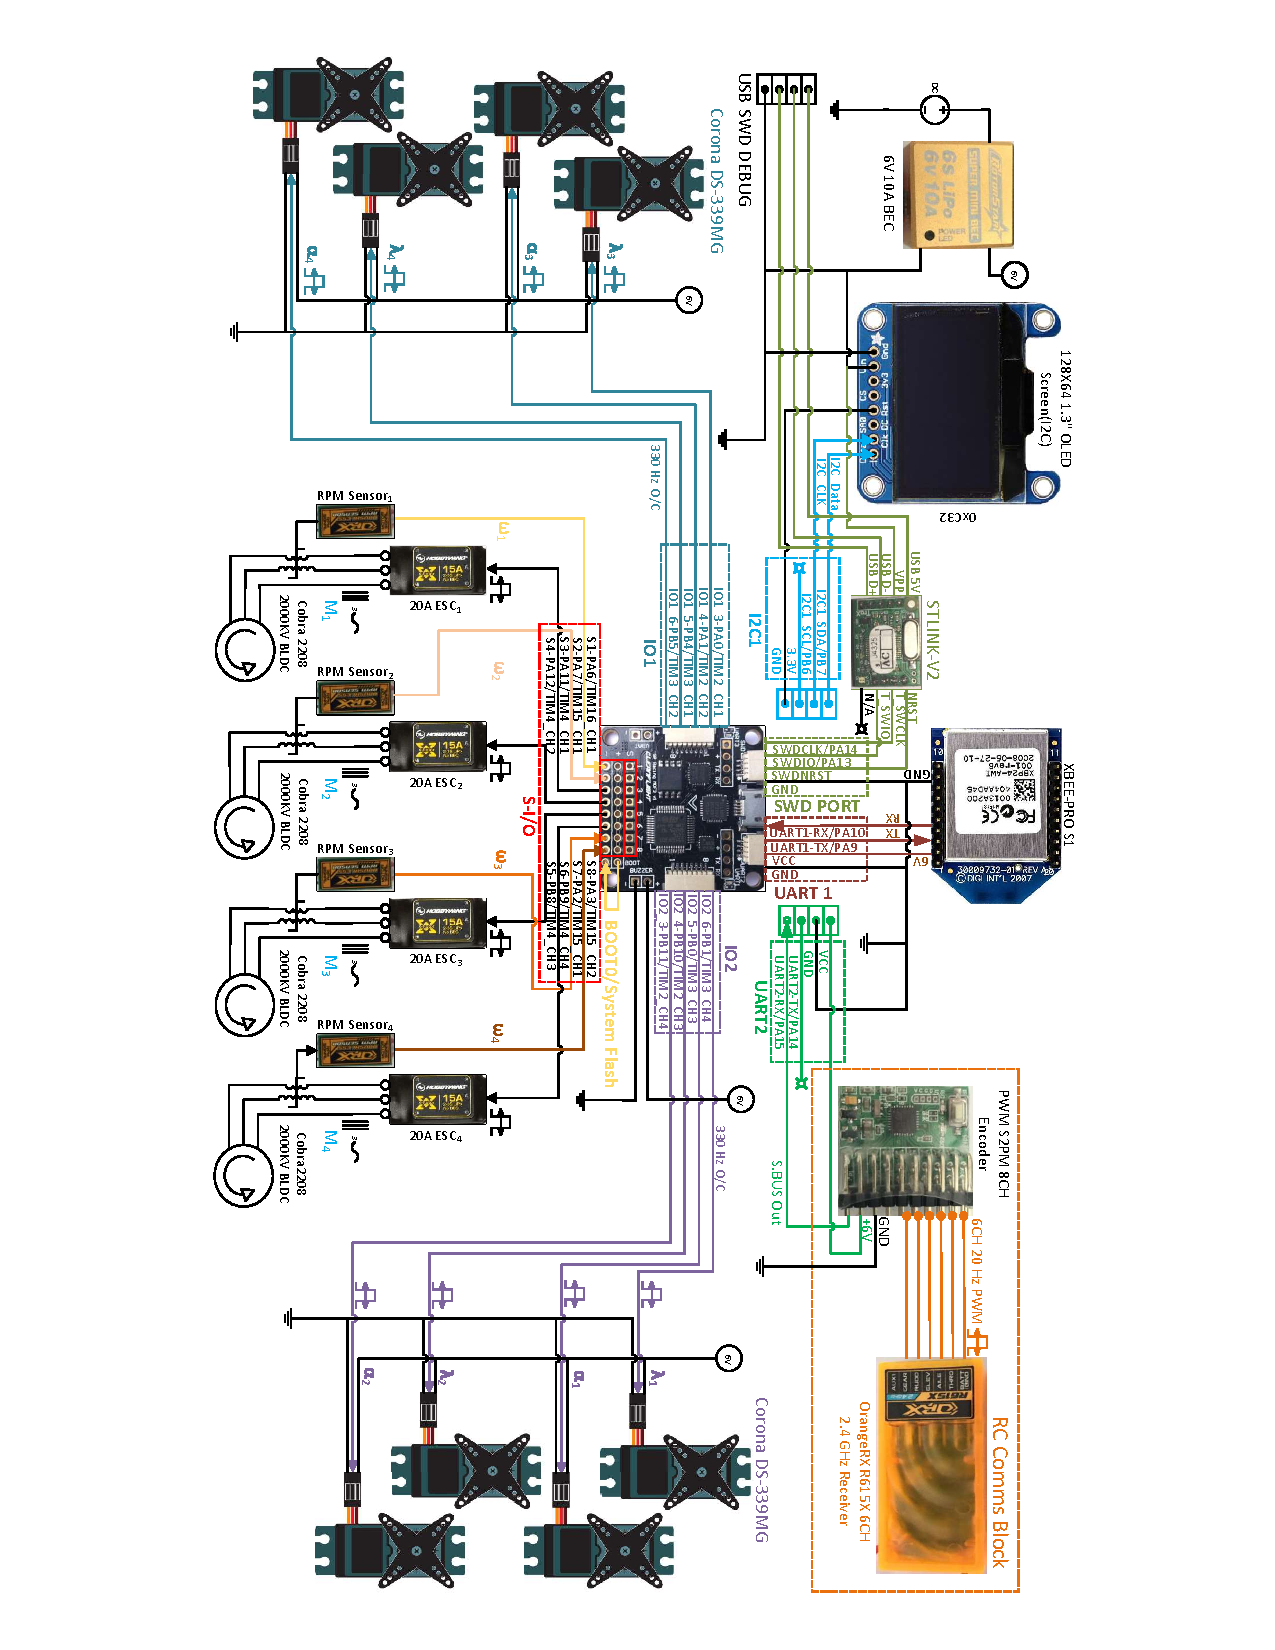
\includegraphics[width=0.95\textwidth]{pdfpages/electrical-schematic.pdf}
\label{fig:electrical-schematic}
\end{minipage}
}
\captionof{figure}{Hardware Schematic Diagram}
}
%-----------------------------------------------------
\newpage
%-----------------------------------------------------
An abstracted hardware diagram for the (electronic) system layout is shown in Fig:\ref{fig:electrical-schematic}. It's an illustration for the connection of different electronic peripherals used to aid the on-board control system. The structure of the autopilot system and control loops are addressed later in Chapter:\ref{ch:flight}. This description aims to provide a brief overview of the specific modules used, their purpose and how they're interfaced. No code structure or control loops are considered yet\ldots
\par
\begin{figure}[htbp]
\begin{subfigure}{0.5\textwidth}
\centering
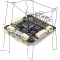
\includegraphics[width=0.9\textwidth]{figs/f3-deluxe}
\caption{SPRacing F3 Deluxe Flight Controller}
\end{subfigure}
\begin{subfigure}{0.5\textwidth}
\centering
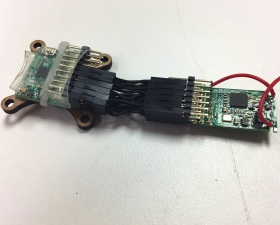
\includegraphics[width=0.9\textwidth]{figs/ppm-sbus}
\caption{SBUS Converter \& 6CH Receiver Modules}
\end{subfigure}
\caption{}
\end{figure}
The entire system is centered around an ARM STM32F303\cite{stm32f303} based $\mu$C. The micro-processor board is a commercial flight control board, specifically an SPRacing F3 Deluxe\cite{spracing}\footnote{CleanFlight opensource software is regularly used for the F3 but its hardware specifications are not openly avaiable.\\The reverse engineered electrical schematic for the board is included in Appendix:\ref{app:deluxe-diagram}}, which has had its bootloader removed and custom firmware, unique to this project, developed for it. That software is later described in Chapter:\ref{ch:flight}; the I/O for all the peripherals are detailed here however. The flight-controller has the following onboard peripherls: an I2C MPU-6050\cite{mpu6050} 6-axis gyroscope \& accelerometer with a connected HMC5883\cite{hmc5883} magnetometer compass, an SPI MS5611\cite{ms5611} barometer and similarly 64 Mb of SPI flash memory. The electrical schematic of those peripherals and the core STM32F303 is detailed in Appendix:\ref{app:deluxe-diagram} but their connection(s) are shown in Fig:\ref{fig:electrical-schematic}. 
\\
\emph{\color{Gray} The combination of above sensors fused for state estimation and their associated algorithms are dealt with in Section:\ref{sec:simulation.state} in Chapter:\ref{ch:simulation}.}
\begin{figure}[hbtp]
\centering
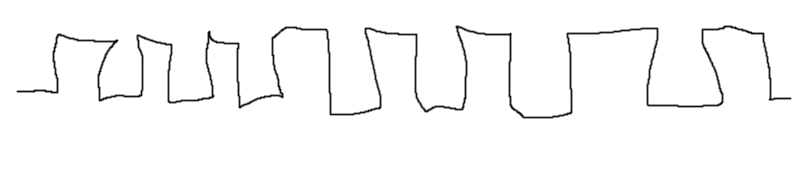
\includegraphics[width=\textwidth]{figs/sbus}
\caption{S.BUS Data Stream}
\label{fig:sbus}
\end{figure}
\\
Two wireless communication peripherals are used. First the system relays full state information, for a complete 6-DOF autopilot system, from a ground control station using 2.4 GHz XBEE S1 module(s)\cite{xbees1}, USART connected. Secondly, an augmented pilot control input system, fail safe and secondary to the autopilot loop, is transmitted through 6 Channel 2.4 GHz R/F comms. The 6 CH received signals, otherwise permeated as six individual 20 KHz PWM signals via an OrangeRx R615x\cite{r615x} receiver, are encoded into a single proprietary S.BUS data stream. 
\newpage
The need for an S.BUS encoder \cite{sbusencoder} comes about as a consequence of the introduction of the 8 additional servos. As a result, there are no longer 6 free additional timer I/O channels which can be allocated for input capture. Encoding the received data to a serial communication protocol means the 6CH data can be processed on a single serial RX line. The S.Bus encoder implements a USART derivative communications standard, Fig:\ref{fig:sbus} shows the sampled data stream used to ascertain the standard's following parameters:
\\
\begin{tabularx}{\textwidth}{|X|c|}
\hline
\begin{minipage}{\textwidth}
\begin{itemize}[itemsep=0em]
\item 8-Bit byte length
\item 25 Bytes per packet
\item Bytes are:
\vspace{-5pt}
\begin{itemize}[itemsep=0em]
\item MSB First
\item 1 start bit
\item 2 stop bits
\item Even parity bit
\item Inverted
\item 100000 baud (bps)
\end{itemize}
\vspace{-5pt}
\item 14 ms idle time between packets
\item Up to 16CH encoded
\item Each channel's data is 11 bits long
\item Channel data is little endian prioritized
\end{itemize}
\end{minipage}
&
\begin{minipage}{\textwidth}
Data packet structure
\end{minipage}
\\
\hline
\end{tabularx}
{\color{red}
The received information of the transmitted 6 channels is filtered through an Infinite-Impulse Response filter. The filters frequency response is as follows: $
y_n = y_{n-1}$. Any referenced signals received are all post filtered data. Filtering for state estimates is separately performed on the Ground Control Station computer.}
\par
Each of the eight digital servo actuators are driven individually from 330 Hz PWM timer output compare channels (TIM2:CH1$\rightarrow$CH4 \& TIM3:CH1$\rightarrow$CH4). Output pulses range from 1ms - 2ms to linearly control the rotary position. The exact range and transfer function is empirically determined next in Subsection:\ref{subsec:proto.design.transfer}. The four 20A brushless DC speed controllers (ESCs) are each driven from a 20 Hz PWM output (TIM4:CH1$\rightarrow$CH4), similarly with 1ms - 2ms pulse widths. There are a total of 12 PWM output compare signals drawn from the $\mu$controller. Servos are powered by a regulated 6V DC 10A power supply \cite{rotorstar} whilst the ESCs switch unregulated 15.1 V DC from an externally tethered power supply. The DC supply could potentially be drawn from an on-board battery bank but that would add significant weight to an already heavy platform.
\par
There's no integrated feedback for instantaneous RPM values from the ESCs. Using discrete OrangeRX BLDC RPM sensors \cite{orangerpm}, that measure switching phases across two of the three motor phases, the exact RPM can be ascertained. The switching signal of a 3-Phase \footnote{Although called BLDC motors, the motors are actually 3-Phase IM motors which, when combined with an ESC, behave in closed loop like BLDC motors.} is:
\begin{equation}
F_{rps}=\frac{2\times F_{poles}}{\text{No. of rotor poles}}~~[Hz]
\end{equation}
The signal produced by the RPM sensors varies a 50\% duty cycle square wave's period, directly proportional to that pole switching frequency. The RPM sensor's output signal is then calibrated to a gain of 7 for the 14 pole BLDC Cobra motors used. That gain is verified with the linear relationship(s) is shown in Figs:\ref{fig:rpm-sensor}. Knowing exact RPM rates means the subsequent thrust and aerodynamic torques for the control plant inputs can be calculated.
\newpage
\begin{figure}[htbp]
\begin{subfigure}{0.5\textwidth}
\centering
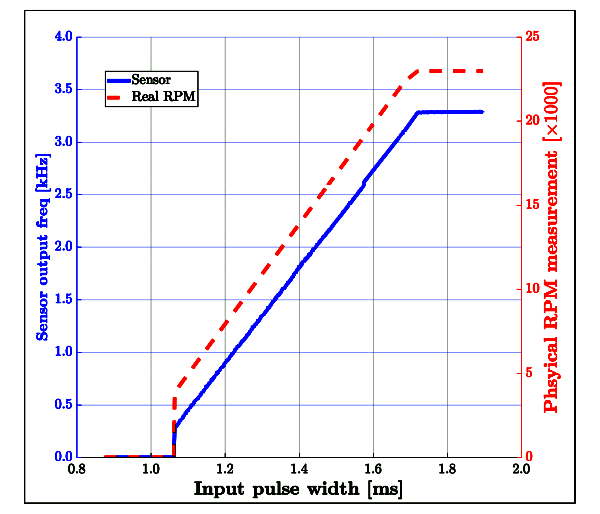
\includegraphics[width=\textwidth]{graphs/rpm-sensor-noload}
\caption{RPM sensor plot - no load}
\label{fig:rpm-sensor-noload}
\end{subfigure}
\begin{subfigure}{0.5\textwidth}
\centering
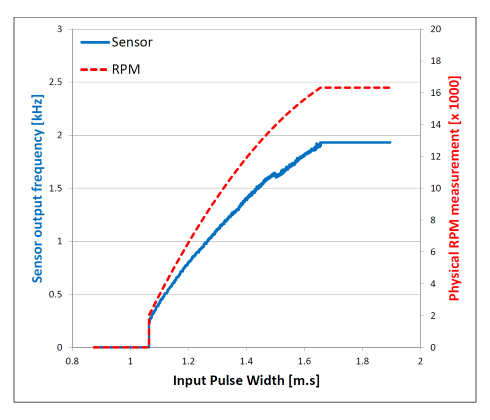
\includegraphics[width=\textwidth]{graphs/rpm-sensor-prop}
\caption{RPM sensor plot - 6" prop}
\label{fig:rpm-sensor-prop}
\end{subfigure}
\caption{}
\label{fig:rpm-sensor}
\end{figure}
\par
The speed controllers, although LDPower 20A devices, were re-flashed with BLHeli\footnote{LDPower 20A ESCs(Fig:\ref{fig:ldpower-20A}) match Hobbywing Xrotor 20A speed controllers (Fig:\ref{fig:xrotor-20A}), they both use SiLabs F396 MCUs. Physical rotational values in the plots Fig:\ref{fig:rpm-sensor} were measured with optical encoders.}\cite{BLHeli} firmware. The custom software on the ESC's $\mu$controller provides greater refinement over parameter configuration like the deflection range of inputs, however, default values were used. The plot in Fig:\ref{fig:rpm-sensor-noload} shows the linear RPM speed line for an unloaded motor, similarly in Fig:\ref{fig:rpm-sensor-prop} shows the plot for a 6-inch prop. It's interesting to note that the loaded speed curve is slightly parabolic, this is from the aerodynamic drag term which is quadratic with respect to rotational velocity, Section:\ref{subsec:dynamics.aero.bem}. Moreover, when the motor is torque loaded by the propeller, the ESC current limits rotational speeds at just over 13 000 RPM. The sensor feedback is used for closed loop RPM control.
\begin{figure}[hbtp]
\begin{subfigure}{0.5\textwidth}
\centering
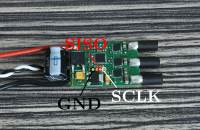
\includegraphics[width=0.9\textwidth]{figs/xrotor-20A}
\caption{XRotor 20A ESC connection guide\cite{xrotor}}
\label{fig:xrotor-20A}
\end{subfigure}
\begin{subfigure}{0.5\textwidth}
\centering
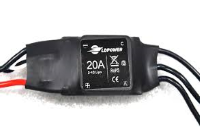
\includegraphics[width=0.9\textwidth]{figs/ldpower-20A}
\caption{LDPower 20A ESC}
\label{fig:ldpower-20A}
\end{subfigure}
\caption{}
\end{figure}
\\
Timers channels are for measuring the varying frequency of the RPM sensors. General purpose Timers 15 (TIM15:CH1$\rightarrow$CH2), 16 (TIM16:CH1) and 17 (TIM17:CH1) are configured to capture the input PWM signal generated by the speed sensors. Included on the I2C communciation line is an I2C O-LED display for debugging and status update purposes.
\par
Any STM32 $\mu$controller is programmed through a dedicated debugging device. The ST-Link V2\cite{st-link} is the current proprietary device which, itself, is a specially programmed STM32F10 chip. The chip connects to the dedicated Serial Wire Debugging ports of the target STM (\emph{SWD-CLK, SWD-IO} \& \emph{SWD-NRST}) and is interfaced via regular USBD+ and USBD- data lines. 
%====================================================
\subsection{Actuator Transfer Functions}
\label{subsec:proto.design.transfer}
%====================================================
\subsubsection*{Servo Transfer Functions}
The full scale deflection of each digital servo is in fact greater than its listed 180\textdegree ~range. Each servo has a rotational range of around 230\textdegree ~(Fig:\ref{fig:servo-range}). The exact characteristics for every servo will differ slightly and so individual transfer functions for each of the 8 servos are used. In the prototype control loop the servos are left in open loop; the major loop controller coefficients are expected to account for minor loop actuator dynamics. With that being said, for such an expectation the simulation would need to accurately represent the servo's response. Seeing that the 180\textdegree ~limitation was a design decision imposed, one of the first points of comparison is the effect such a constraint would have on the feasible operational regions. The control algorithms developed in Chapter:\ref{ch:control} are first tested with an ideal, continuous rotation servo actuator with similar rate limits and transfer characteristics.
\begin{figure}[htbp]
\centering
\begin{subfigure}{0.49\textwidth}
\centering
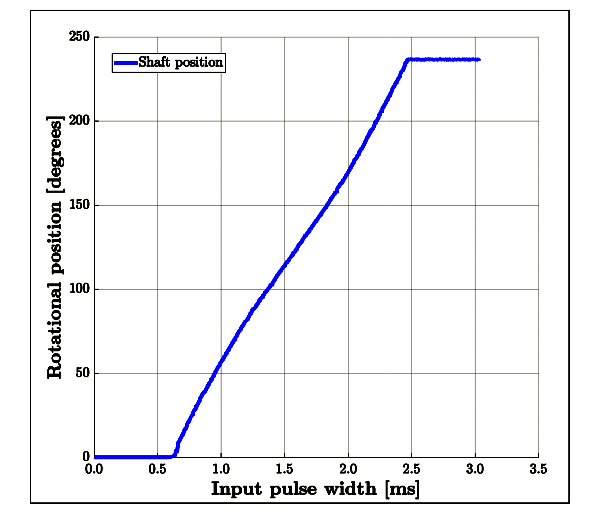
\includegraphics[width=\textwidth]{graphs/servo-range}
\caption{DS339-MG Full Range}
\label{fig:servo-range}
\end{subfigure}
\begin{subfigure}{0.49\textwidth}
\centering
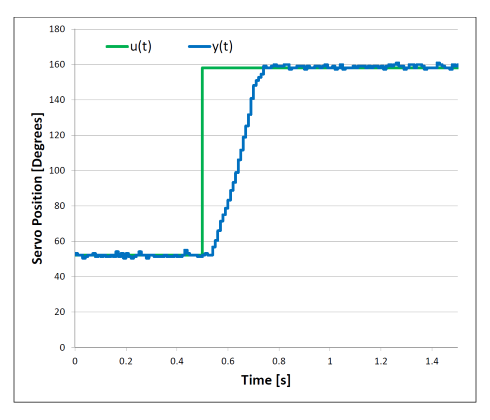
\includegraphics[width=\textwidth]{graphs/servo-step}
\caption{DS339-MG Step Response}
\label{fig:servo-step}
\end{subfigure}
\caption{}
\end{figure}
\par
For the servo whose data is plotted in Fig:\ref{fig:servo-range}, the relationship between the pulse-width input $x~~[m.s]$ and rotational output position $y~~degrees$ is given by:
\begin{equation}\label{eq:servo-range}
y(x)=
\begin{cases}\begin{array}{ll}
0\text{\textdegree} & ~~x<0.64~m.s\\
127.78x-81.78 & ~~0.64~m.s \leq x \leq 2.44~m.s\\
230\text{\textdegree} & ~~x>2.44~m.s\\
\end{array}
\end{cases}
\end{equation}
Although the equation Eq:\ref{eq:servo-range} is changed such that 0\textdegree ~is taken at around a 50\% input and the operational range is $\pm 90$\textdegree . The servo is mechanically rate limited to $60\text{\textdegree}/0.15s$ or $400 RPS$ with a dead time of $0.142~m.s$.
A servo has a (\emph{critically damped}) second order transfer function$^{\dagger}$:
\begin{equation}
G(s)=\frac{7.144}{s^2+3.744s+7.189}e^{-0.142\times 10^{-3}s}
\end{equation}
Whose transfer block has the following structure, including non-linearities:

\subsubsection*{Motor RPM Transfer Functions}


%====================================================
